\chapter{总结与展望}

\section{本文工作总结}
    本文试图解决的问题是,在眼底黄斑区OCT图像中,在仅有类别标签的中等规模数据集上,训练一个模型,使得它在输出预测的类别标签的同时,提供像素级别的病变位置推测信息。

    算法的基本数学动机来源于欧拉距离下的最小二乘拟合。但为了解决高维、相关性等问题,对提取的特征向量做了如下预设:减少相关性,提高判别性的要求,同时,为了在分类之后可以给出空间信息,还要求给出一种方法,使得提取的特征向量被映射回原像素空间,即要求特征的可逆性。为满足这些性质,本文合理选取了简明经典的数学工具,得到了特征向量,并重建了健康图像进而推断病变位置,并对以上过程给出了具体算法。

    设计实验验证了根据算法提取的特征向量初步符合设计之初要求的几条性质。在分类问题上取得了有竞争力的准确率表现的同时,还输出了视觉上可接受的预测病态位置信息。


\section{未来工作展望}
    本工作的分类准确性还与最前沿的工作有差距,虽然本工作的初衷不是提高分类准确性,但是提取的特征向量分类越准确,特征的判别性就越强,对于病态定位越有帮助。

    在病态定位任务中,虽然得到了大部分视觉可接受的结果,但是仍然有一些失败的例子,如图~\ref{fig:fail}是较典型的失败例子。这可能是因为病变导致形态变化过大,使得在特征空间上,该点脱离健康特征子空间过远,被映射到了一个与实际图像差距较大的图像的特征向量上。纠正这种情况,可能从两方面改进:首先,提高数据预处理的能力,使得这种形态变化过大的图片也可以经适度形变后对齐;其次,引入多尺度空间的特征提取,使得适当降低对于位移的敏感度。

    \begin{figure}[H] % use float package if you want it here
      \centering
      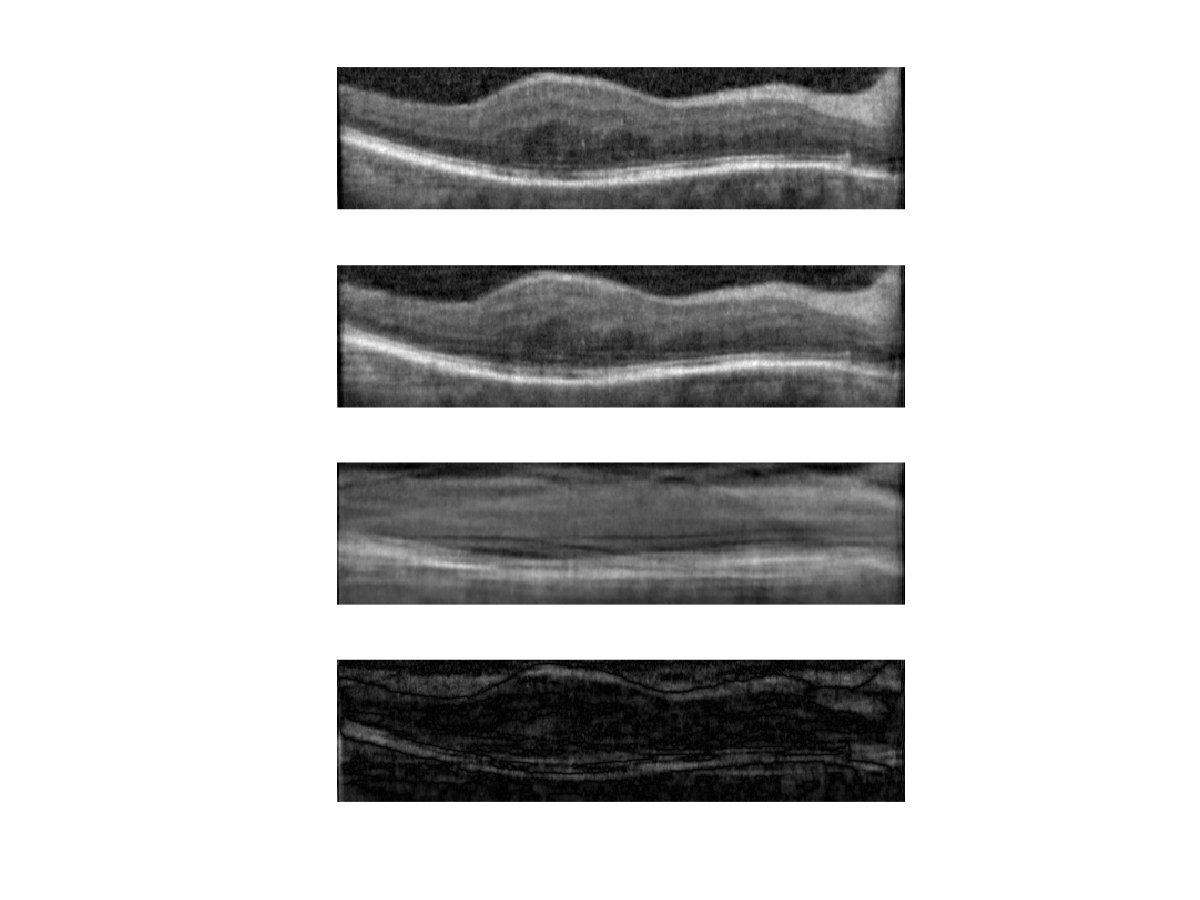
\includegraphics[width=\textwidth]{fail}
      \caption{典型失败例子}
      \label{fig:fail}
    \end{figure}

    尽管工作还存在改进的地方,但是,它为只有类别标注的中等规模的眼底视网膜黄斑区OCT成像预测病态位置信息问题,提供了一种简洁的设计思路,被证明是一种较有效的方法。

